\typeout{NT FILE chapter5.tex}
\chapter{Training the model on more data} \label{new_data_train}
\paragraph{}
In section \ref{rs_data_collection} JP2 data is introduced as a larger dataset sourced to address the issues of bias in data collection. This chapter is dedicated to the evaluation of the impact of using such data on the model fine-tuned on the smaller GEE dataset through the experiments in Chapter \ref{experiments_chapter}.

\section{Using the weights of previous model to train on new data}
\paragraph{}
The model was frozen using the best hyperparameters at the end of the Chapter \ref{experiments_chapter} and the model was trained on new data using those weights, this will be compared with the performance of training the model from scratch on new data in section \ref{new_data_train}, the same ES strategy will be used for this experiment to prevent overfitting.

\begin{figure}[hbt!]
    \centering
    % \begin{minipage}[c]{0.45\linewidth}
    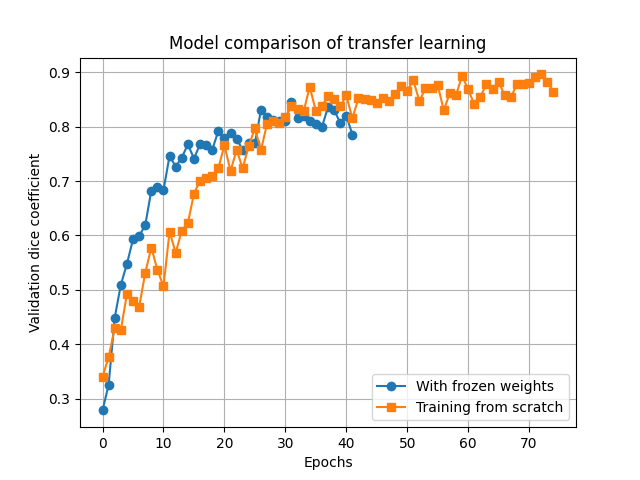
\includegraphics[width=0.75\linewidth]{transfer learning_Validation dice coefficient.png}
    \caption{Retraining with frozen weights Dice Coefficient comparison}
    \label{rt_dice}
        % \end{minipage}
    %     \hfill
    % \begin{minipage}[c]{0.45\linewidth}
    %     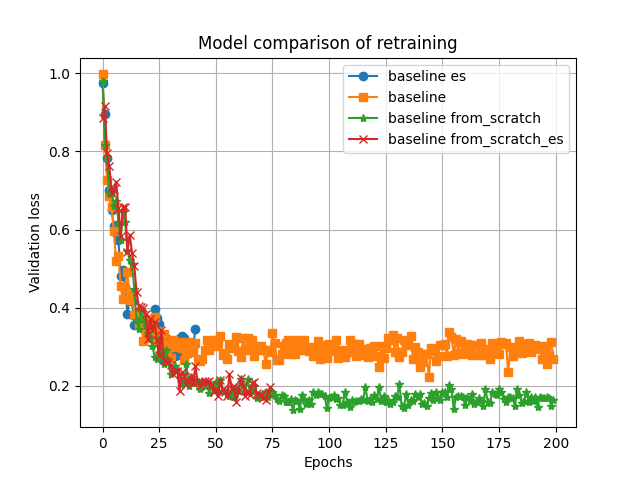
\includegraphics[width=\textwidth]{retraining_Validation loss.png}
    %     \caption{Retraining with frozen weights loss comparison}
    %     \label{rt_loss}
    % \end{minipage}
\end{figure}

Using the frozen weights did not improve model performance, it had the opposite effect which is expected since the original model has a smaller dataset than the one it was trained on now. It can be seen from Figure \ref{rt_dice} that up to 20 epochs the transfer learning by using frozen weights from the model trained on less data is performing better than the model training from scratch. 

Early stopping is also triggered in the model using frozen weights around 30 epochs before the model being trained from scratch, which makes sense since when there is less data the model has a greater likelihood of overfitting.

\section{Training the model from scratch on new data} \label{new_data_fs}
\subsection{Comparison with the GEE dataset model - same parameters}
\paragraph{}
With the same model architecture and hyperparameters as in the previous Chapter, the DL model was trained on the \textit{JP2 data} for the same number of epochs to evaluate the effect of using more data on the model performance.

\begin{figure}[hbt!]
    % \begin{minipage}[c]{0.45\linewidth}
    %     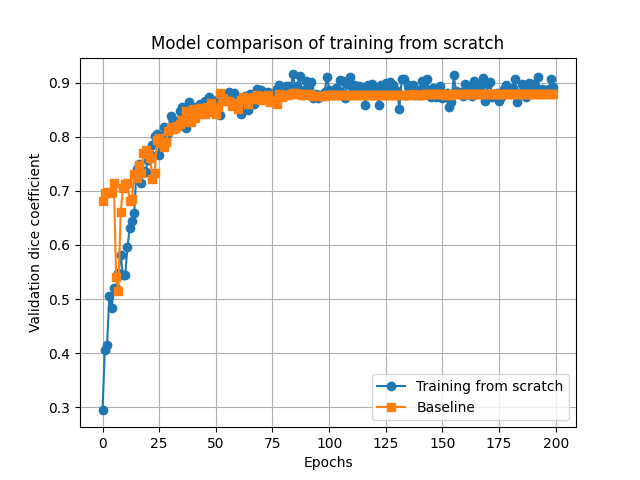
\includegraphics[width=\linewidth]{training from scratch_Validation dice coefficient.png}
    %     \caption{Retraining from scratch dice coefficient comparison}
    %     \label{fs_dice}
    %     \end{minipage}
    %     \hfill
    % \begin{minipage}[c]{0.45\linewidth}
    \centering
    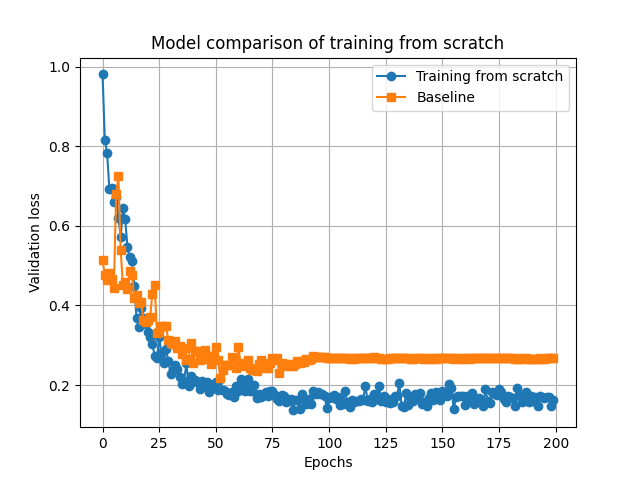
\includegraphics[width=0.75\textwidth]{training from scratch_Validation loss.png}
    \caption{Retraining from scratch Loss comparison}
    \label{fs_loss}
    % \end{minipage}
\end{figure}
\paragraph{}
As can be seen from Figure \ref{fs_loss} the model trained on more data has a lower validation loss consistently after 20 epochs despite initialising with a higher validation loss, which shows it's better performance. 

In terms of evaluation metrics, it can be seen from Table \ref{tab_fs} that the improvement in performance is the most evident in the Test dataset where there is an improvement of 0.08 in the dice coefficient metric when using Early stopping (ES) to prevent overfitting.

\begin{table}[ht] 
    \begin{center}
    \begin{tabular}{ccccccc} 
    \toprule
       & \multicolumn{3}{c}{Dice Coefficient}     & \multicolumn{3}{c}{Loss} \\
    Model type & Validation & Training & Test & Validation    & Training    & Test   \\ \midrule
    \rowcolor{lightgray}
    Training from scratch & 0.89 & 0.96 & 0.88 & 0.16 & 0.05 & 0.28  \\ Training from scratch with ES & 0.86 & 0.94 & 0.86 & 0.2 & 0.08 & 0.3  \\ Baseline model & 0.88 & 0.97 & 0.82 & 0.27 & 0.05 & 0.27  \\ Baseline Model with ES & 0.88 & 0.96 & 0.78 & 0.26 & 0.07 & 0.33  \\
    \bottomrule
    \end{tabular}
  \end{center} 
  \caption{Retraining on new data comparison of Dice coefficient and Loss}\label{tab_fs}
\end{table}

\subsection{Hyperparameter tuning from scratch} \label{hp_new_data}
\paragraph{}
What works well for a dataset in terms of hyperparameters may not work well for another, especially when there is a considerable difference in sample size. With this in mind, hyperparameter tuning using random search was performed on the new data with the following parameter variations using the same Early Stopping strategy as before, restoring the weights of the best performing epoch \gls{w.r.t.} Validation Loss:

\begin{itemize}
    \item{Learning Rate: 0.0001 and 0.001}
    \item{Optimiser: RMSprop,Adam and Nadam}
    \item{Loss Function: CE Dice Loss}
    \item{Batch Size: 1 and 10}
    \item{Activation Function: ELU}
    \item{Initialisation Method: He Normal}
\end{itemize}
\paragraph{}
Results were logged using Tensorboard, the best validation dice coefficient combinations of hyperparameters are shown in Figure \ref{hp}, the best hyperparameters for the JP2 data were batch size of 10, \gls{RMSProp} optimiser and learning rate of 0.001.

\begin{figure}[hbt!]
    \centering
    % \begin{minipage}[c]{0.45\linewidth}
    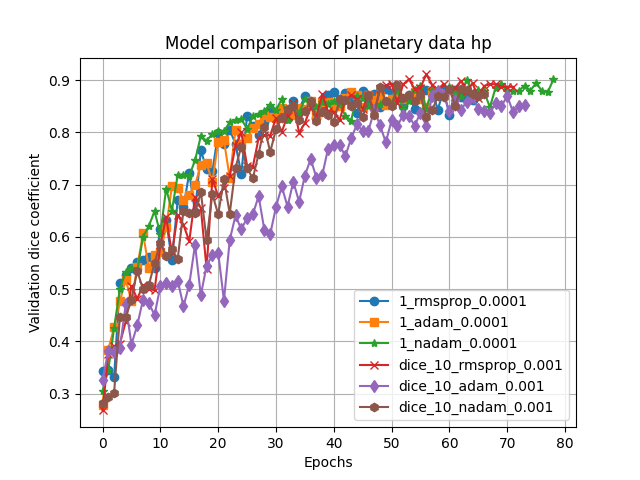
\includegraphics[width=0.75\linewidth]{planetary data hp_Validation dice coefficient.png}
    \caption{Subset of hyperparameter experiments with new data Validation dice coefficient}
    \label{hp}
        % \end{minipage}
    %     \hfill
    % \begin{minipage}[c]{0.45\linewidth}
    %     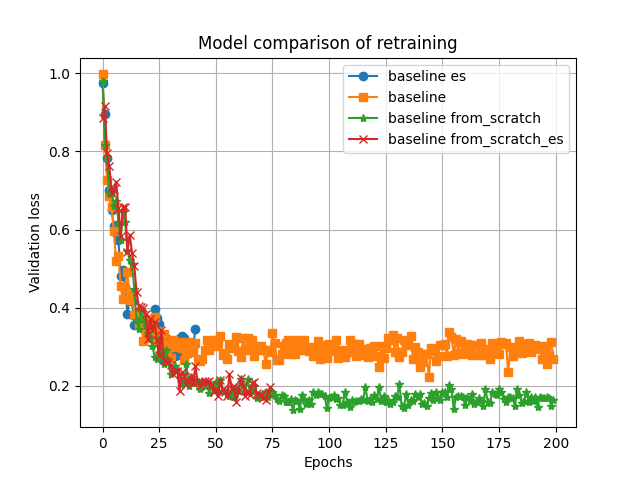
\includegraphics[width=\textwidth]{retraining_Validation loss.png}
    %     \caption{Retraining with frozen weights loss comparison}
    %     \label{rt_loss}
    % \end{minipage}
\end{figure}
\paragraph{}
As it can be seen from Table \ref{tab_hp} the difference in performance with regards to the Validation Dice Coefficient is marginal between the different hyperparameter combinations, showing that the previous experiments in Chapter \ref{experiments_chapter} provided good insights that generally apply to a different bigger dataset.

\begin{table}[ht!] 
    \begin{center}
    \begin{tabular}{ccccccc} 
    \toprule
       & \multicolumn{3}{c}{Dice Coefficient}     & \multicolumn{3}{c}{Loss} \\
    Hyperparameter combination & Validation & Training & Test & Validation    & Training    & Test   \\ \midrule
%\rowcolor{lightgray}
    1 rmsprop 0.0001 & 0.86 & 0.94 & 0.93 & 0.2 & 0.07 & 0.15  \\ 1 adam 0.0001 & 0.87 & 0.93 & 0.91 & 0.19 & 0.09 & 0.14  \\ 1 nadam 0.0001 & 0.86 & 0.93 & 0.76 & 0.2 & 0.09 & 0.22  \\ \rowcolor{lightgray}10 rmsprop 0.001 & 0.91 & 0.96 & 0.95 & 0.13 & 0.05 & 0.11  \\ 10 adam 0.001 & 0.6 & 0.68 & 0.64 & 0.55 & 0.44 & 0.36  \\ 10 nadam 0.001 & 0.59 & 0.72 & 0.84 & 0.56 & 0.38 & 0.33  \\
\bottomrule
    \end{tabular}
  \end{center} 
  \caption{Hyperparameter combinations comparison of Dice Coefficient and Loss}\label{tab_hp}
\end{table}
